\input{mmd-mavrldoc-header}
\usepackage{multirow}
\usepackage{pdfpages}
\def\mytitle{NANO106 Handout 4 - Point Groups}
\def\latexmode{mavrldoc}

\begin{document}
\chapter{NANO106 Handout 4 - Point Group Summary and Determination}
\begin{table}[h]
\centering
\small
  \begin{tabular}{lcccc}
    \hline
	\textbf{Crystal}           & \textbf{Laue Class}             & \multicolumn{2}{l}{\textbf{Hermann-Mauguin}} & \textbf{Schoenflies}\\
   	\textbf{System}            &                                 & \textbf{Full} & \textbf{Short }              & \\
   	\hline
   	\hline
   	\multirow{2}{*}{Triclinic} & \multirow{2}{*}{$\overline{1}$} & $1$ & $1$ & $C_1$\\
                               &                                 & $\overline{1}$ & $\overline{1}$ & $C_i = S_2$ \\
    \hline
    \multirow{3}{*}{Monoclinic} & \multirow{3}{*}{$\displaystyle \frac{2}{m}$} & $2$ & $2$ & $C_2$\\
                               &                                 & $m$ & $m$ & $C_s = C_{1h}$ \\
                               &                                 & $\displaystyle \frac{2}{m}$ & $\displaystyle \frac{2}{m}$ & $C_{2h}$ \\[1.5ex]
    \hline 
    \multirow{3}{*}{Orthorhombic} & \multirow{3}{*}{$mmm$} & $222$ & $222$ & $D_2$\\
                               &                           & $mm2$ & $mm2$ & $C_{2v}$ \\
                               &                           & $\displaystyle \frac{2}{m}\frac{2}{m}\frac{2}{m}$ & $mmm$ & $D_{2h}$ \\[1.5ex]
    \hline
    \multirow{7}{*}{Tetragonal} & \multirow{3}{*}{$\displaystyle \frac{4}{m}$} & $4$ & $4$ & $C_4$\\
                               &                                 & $\overline{4}$ & $\overline{4}$ & $S_4$ \\
                               &                                 & $\displaystyle \frac{4}{m}$ & $\displaystyle \frac{4}{m}$ & $C_{4h}$ \\[1.5ex]
                               \cline{2-5}
							  & \multirow{4}{*}{$\displaystyle \frac{4}{m}mm$} & $422$ & $422$ & $D_4$\\
                               &                                 & $4mm$ & $4mm$ & $C_{4v}$ \\
                               &                                 & $\overline{4}2m$ & $\overline{4}2m$ & $D_{2d}$ \\ 
                               &                                 & $\displaystyle \frac{4}{m}\frac{2}{m}\frac{2}{m}$ & $\displaystyle \frac{4}{m}mm$ & $D_{4h}$ \\ [1.5ex]
    \hline
    \multirow{5}{*}{Trigonal } & \multirow{2}{*}{$\overline{3}$} & $3$ & $3$ & $C_3$\\
                               &                                 & $\overline{3}$ & $\overline{3}$ & $C_{3i}$ \\
                               \cline{2-5}
							  & \multirow{3}{*}{$\overline{3}m$} & $32$ & $32$ & $D_3$\\
                               &                                 & $3m$ & $3m$ & $C_{3v}$ \\
                               &                                 & $\overline{3}m$ & $\overline{3}m$ & $D_{3d}$ \\ 
    \hline
    \multirow{7}{*}{Hexagonal} & \multirow{3}{*}{$\displaystyle \frac{6}{m}$} & $6$ & $6$ & $C_6$\\
                               &                                 & $\overline{6}$ & $\overline{6}$ & $C_{3h}$ \\
                               &                                 & $\displaystyle \frac{6}{m}$ & $\displaystyle \frac{6}{m}$ & $C_{6h}$ \\[1.5ex]
                               \cline{2-5}
							  & \multirow{4}{*}{$\displaystyle \frac{6}{m}mm$} & $622$ & $622$ & $D_6$\\
                               &                                 & $6mm$ & $6mm$ & $C_{6v}$ \\
                               &                                 & $\overline{6}m2$ & $\overline{6}m2$ & $D_{3h}$ \\ 
                               &                                 & $\displaystyle \frac{6}{m}\frac{2}{m}\frac{2}{m}$ & $\displaystyle \frac{6}{m}mm$ & $D_{6h}$ \\  [1.5ex]
    \hline
    \multirow{5}{*}{Cubic}    & \multirow{2}{*}{$m\overline{3}$} & $23$ & $23$ & $T$\\
                               &                                 & $\displaystyle \frac{2}{m}\overline{3}$ & $m\overline{3}$ & $T_h$ \\
                               \cline{2-5}
							  & \multirow{3}{*}{$m\overline{3}m$} & $432$ & $432$ & $O$\\
                               &                                 & $\overline{4}3m$ & $\overline{4}3m$ & $T_d$ \\
                               &                                 & $\displaystyle \frac{4}{m}\overline{3}\frac{2}{m}$ & $m\overline{3}m$ & $O_h$ \\ [1.5ex]
    \hline  
  \end{tabular}
\end{table}


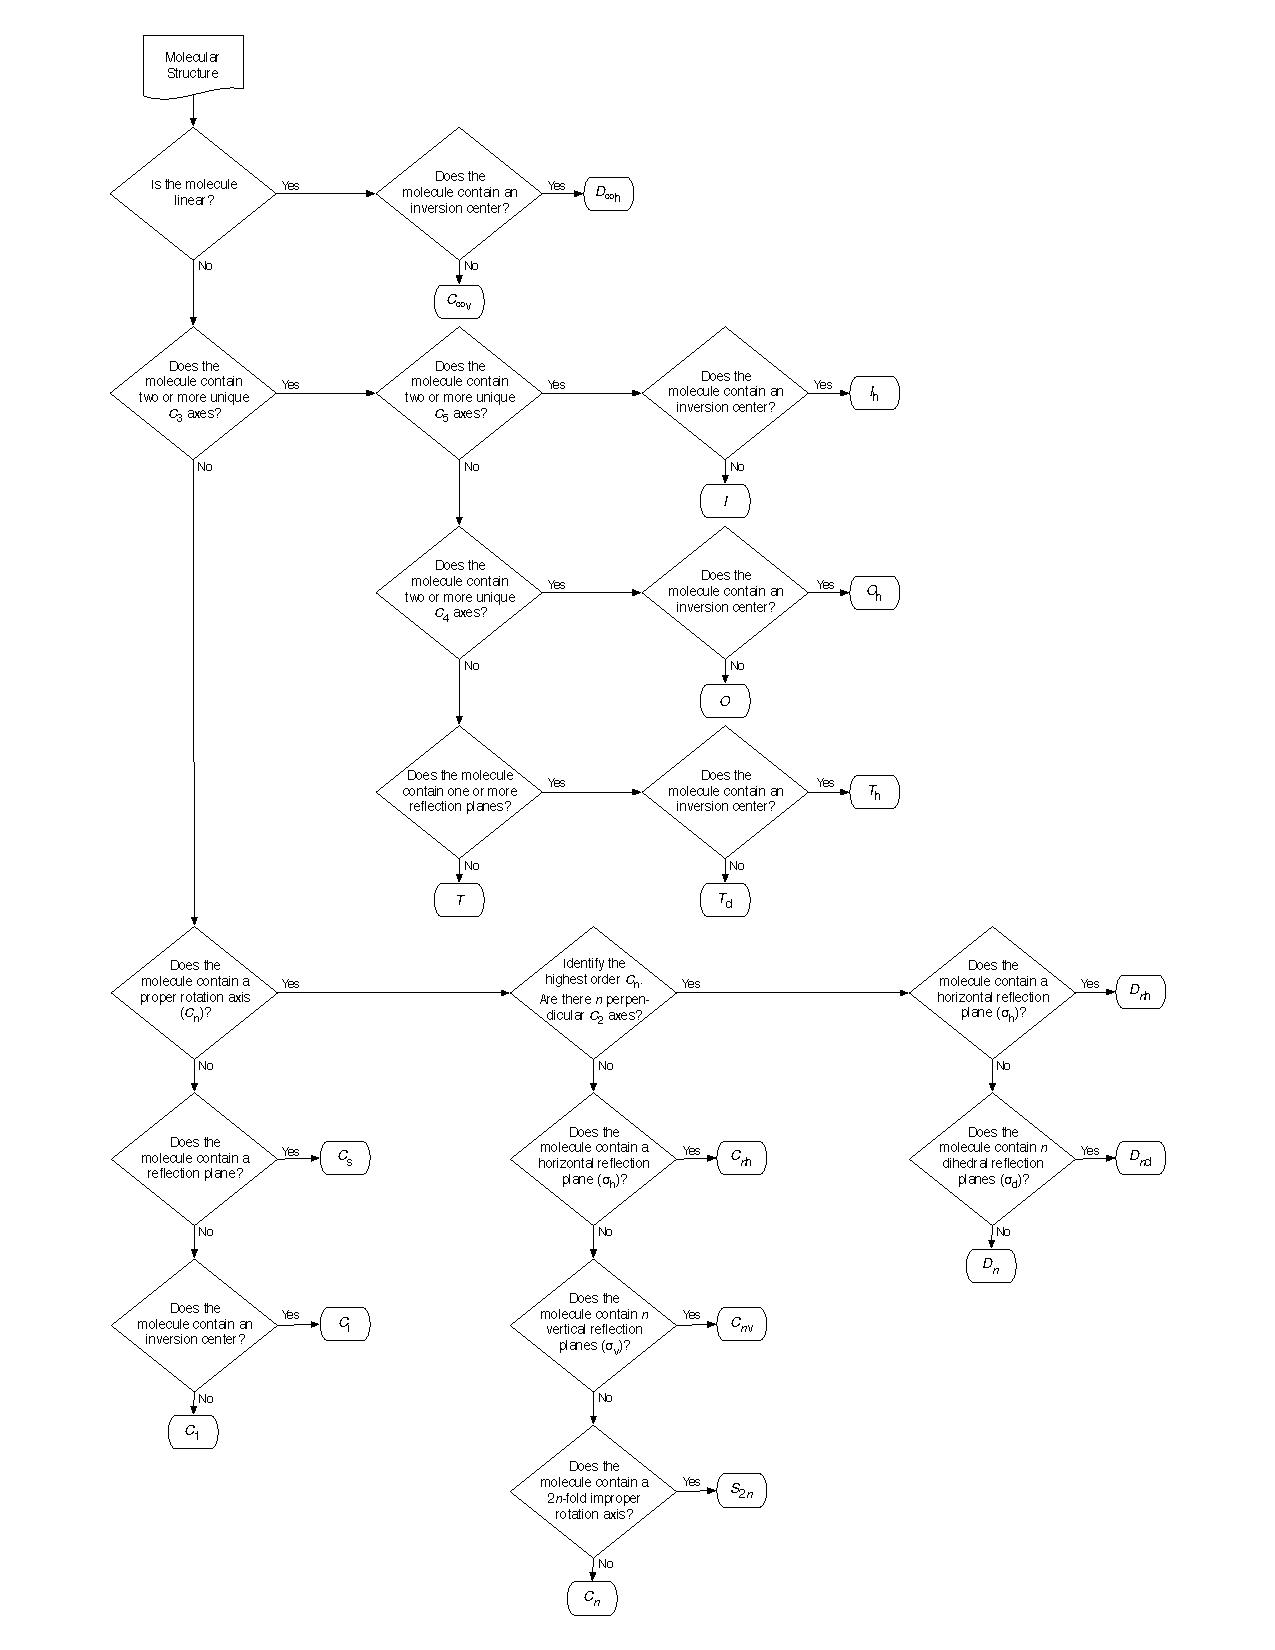
\includepdf[pages={1}]{PGFlowChart.pdf}

\end{document}